\documentclass[10pt]{article}  
\usepackage{hyperref}
\usepackage{lmodern}
\usepackage{amsmath,amsfonts,amssymb}
\usepackage{color}
\usepackage{latexsym}
\usepackage{graphicx}
\usepackage{amssymb}
\usepackage{polynom}
\usepackage{qtree}
\usepackage{graphicx}
\usepackage{tikz-qtree}
\usepackage{tkz-graph}
\usepackage{tikzpagenodes}
\usepackage{wasysym}
\usepackage{tikz}
\usepackage{color}
\usepackage{hyperref}
\usepackage{tikz}
\usepackage[ngerman]{babel}   
\usepackage{xltxtra}
\setmainfont{Quicksand-Regular.otf}[
	Path = src/fonts/,
	BoldFont = Quicksand-Bold.otf ,
	ItalicFont     = Quicksand-Italic.otf,
	BoldItalicFont = Quicksand-BoldItalic.otf]
\setsansfont{Karla-Regular.ttf}[
	Path = src/fonts/,
	BoldFont = Karla-Bold.ttf ,
	ItalicFont     = Karla-Italic.ttf,
	BoldItalicFont = Karla-BoldItalic.ttf]
\usepackage[a6paper, left=1cm,right=1cm,top=1cm,bottom=1cm]{geometry}
\setlength{\parindent}{0em} 
\usepackage[pangram]{blindtext}
\providecommand{\tightlist}{%
  \setlength{\itemsep}{0pt}\setlength{\parskip}{0pt}}
\setlength{\parindent}{0cm}


\newcommand{\filmname}{\@empty}
\newcommand{\filmbild}{\@empty}
\newcommand{\filmbeschreibung}{\@empty}
\newcommand{\filmdatum}{\@empty}
\newcommand{\filmuhrzeit}{\@empty}

\begin{document}
\def \filmname {FILMTITEL}
\def \filmbeschreibung {\vspace{1cm}BESCHREIBUNG \blindtext}
\def \filmdatum {DATUM}
\def \filmuhrzeit {UHRZEIT}
\def \filmbild {src/figures/beispielbild.jpg}

%\begin{landscape}
\pagestyle{empty}
\begin{tikzpicture}[remember picture,overlay]
   \node[inner sep=0pt, rotate=-20] at ([xshift=-.15\textwidth-.5cm, yshift=-.15\textwidth+.2cm]current page.north east)
              {
\includegraphics[width=.3\textwidth, height=.3\textwidth]{src/figures/LogoGefuelltOhneRahmen}};
\end{tikzpicture}
\begin{tikzpicture}[remember picture,overlay]
	\foreach \i in {1,...,100}
	{
   		\draw [draw=black, fill=white, line width=.6mm] ([xshift=0.03cm,yshift=-0.03cm-\i*0.3cm]current page.north west) rectangle ++(0.3,0.3);
   		\draw [draw=black, fill=white, line width=.6mm] ([xshift=-0.32cm,yshift=-0.03cm-\i*0.3cm]current page.north east) rectangle ++(0.3,0.3);
   		\ifnum \paperheight<\i*0.3
  			\breakforeach
   		\fi
   	}
%	\draw [draw=black, fill=white, line width=.6mm] ([xshift=0.33cm,yshift=-6.5cm]current page.north west) -- ([xshift=-0.32cm,yshift=-6.5cm]current page.north east);
	\draw [draw=black, fill=white, line width=.9mm] ([xshift=0.33cm,yshift=-\paperheight+.3cm]current page.north west) -- ([xshift=-0.32cm,yshift=-\paperheight+.3cm]current page.north east);
	\draw [draw=black, fill=white, line width=.9mm] ([xshift=0.33cm,yshift=-.2cm]current page.north west) -- ([xshift=-0.32cm,yshift=-.2cm]current page.north east);
\end{tikzpicture}
\begin{tikzpicture}[remember picture,overlay]
   \node[inner sep=0pt] at ([xshift=.25\textwidth+1cm, yshift=.25\textheight+1cm]current page.south west)
              {\includegraphics[width=.5\textwidth, height=0.5\textheight]{\filmbild}};
\end{tikzpicture}
\vspace{-.5cm}
\begin{flushleft}
{\LARGE \filmname}
\end{flushleft}
\vspace{.5cm}
{\sffamily \filmbeschreibung}
\vfill
\begin{flushright}
\begin{Large}
Am \filmdatum\vspace{.5cm}\\
Um \filmuhrzeit\vspace{.5cm}\\
Im K.A.F.F.\vspace{1.5cm}\\
\end{Large}
\end{flushright}

%\end{landscape}
\newpage
\pagestyle{empty}
\begin{tikzpicture}[remember picture,overlay]
   \node[inner sep=0pt] at ([xshift=-0cm, yshift=2cm]current page.center)
              {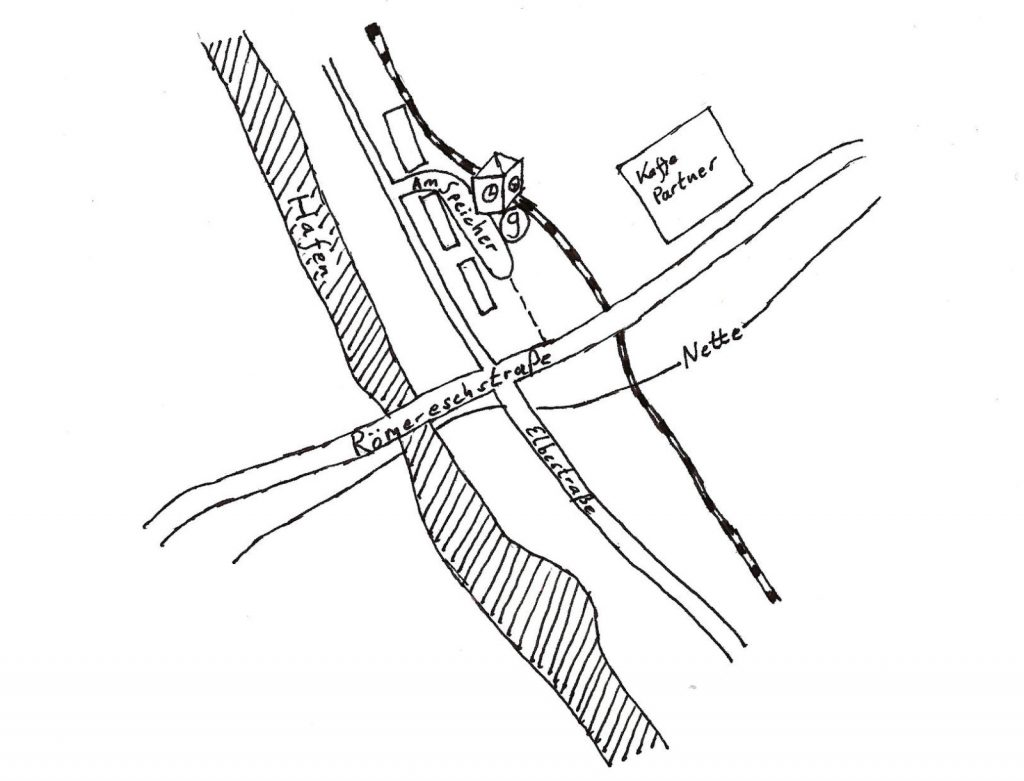
\includegraphics[width=0.9\textheight]{src/figures/AnfahrtPetersburgRot.jpg}};
\end{tikzpicture}
\begin{tikzpicture}[remember picture,overlay]
	\foreach \i in {1,...,100}
	{
   		\draw [draw=black, fill=white, line width=.6mm] ([xshift=0.03cm,yshift=-0.03cm-\i*0.3cm]current page.north west) rectangle ++(0.3,0.3);
   		\draw [draw=black, fill=white, line width=.6mm] ([xshift=-0.32cm,yshift=-0.03cm-\i*0.3cm]current page.north east) rectangle ++(0.3,0.3);
   		\ifnum \paperheight<\i*0.3
  			\breakforeach
   		\fi
   	}
%  	\draw [draw=black, fill=white, line width=.6mm] ([xshift=0.03cm,yshift=5cm]current page.north west) -- ([xshift=-0.32cm,yshift=5cm]current page.north east);
	\draw [draw=black, fill=white, line width=.9mm] ([xshift=0.33cm,yshift=-\paperheight+.3cm]current page.north west) -- ([xshift=-0.32cm,yshift=-\paperheight+.3cm]current page.north east);
	\draw [draw=black, fill=white, line width=.9mm] ([xshift=0.33cm,yshift=-.2cm]current page.north west) -- ([xshift=-0.32cm,yshift=-.2cm]current page.north east);
\end{tikzpicture}

\vfill
\begin{center}
\begin{footnotesize}
Kino am fantastischen Freihafen\vspace{1em}\\
Kulturverein Petersburg e.V.\\
Am Speicher 9\\
49090 Osnabrück\vspace{1em}\\
\url{http://freiraum-petersburg.de/}\\
\url{https://de-de.facebook.com/freiraumpetersburg}
\end{footnotesize}
\end{center}

\end{document}

